\section{Compression}

\addtocounter{framenumber}{1}
\begin{frame}[standout]
    \Large
    Note: Most of these techniques have been demonstrated to work not just for
    transformer networks. Chances are good they work in your case too.
\end{frame}

\subsection{Quantization}
\begin{frame}[c]{Quantization}
    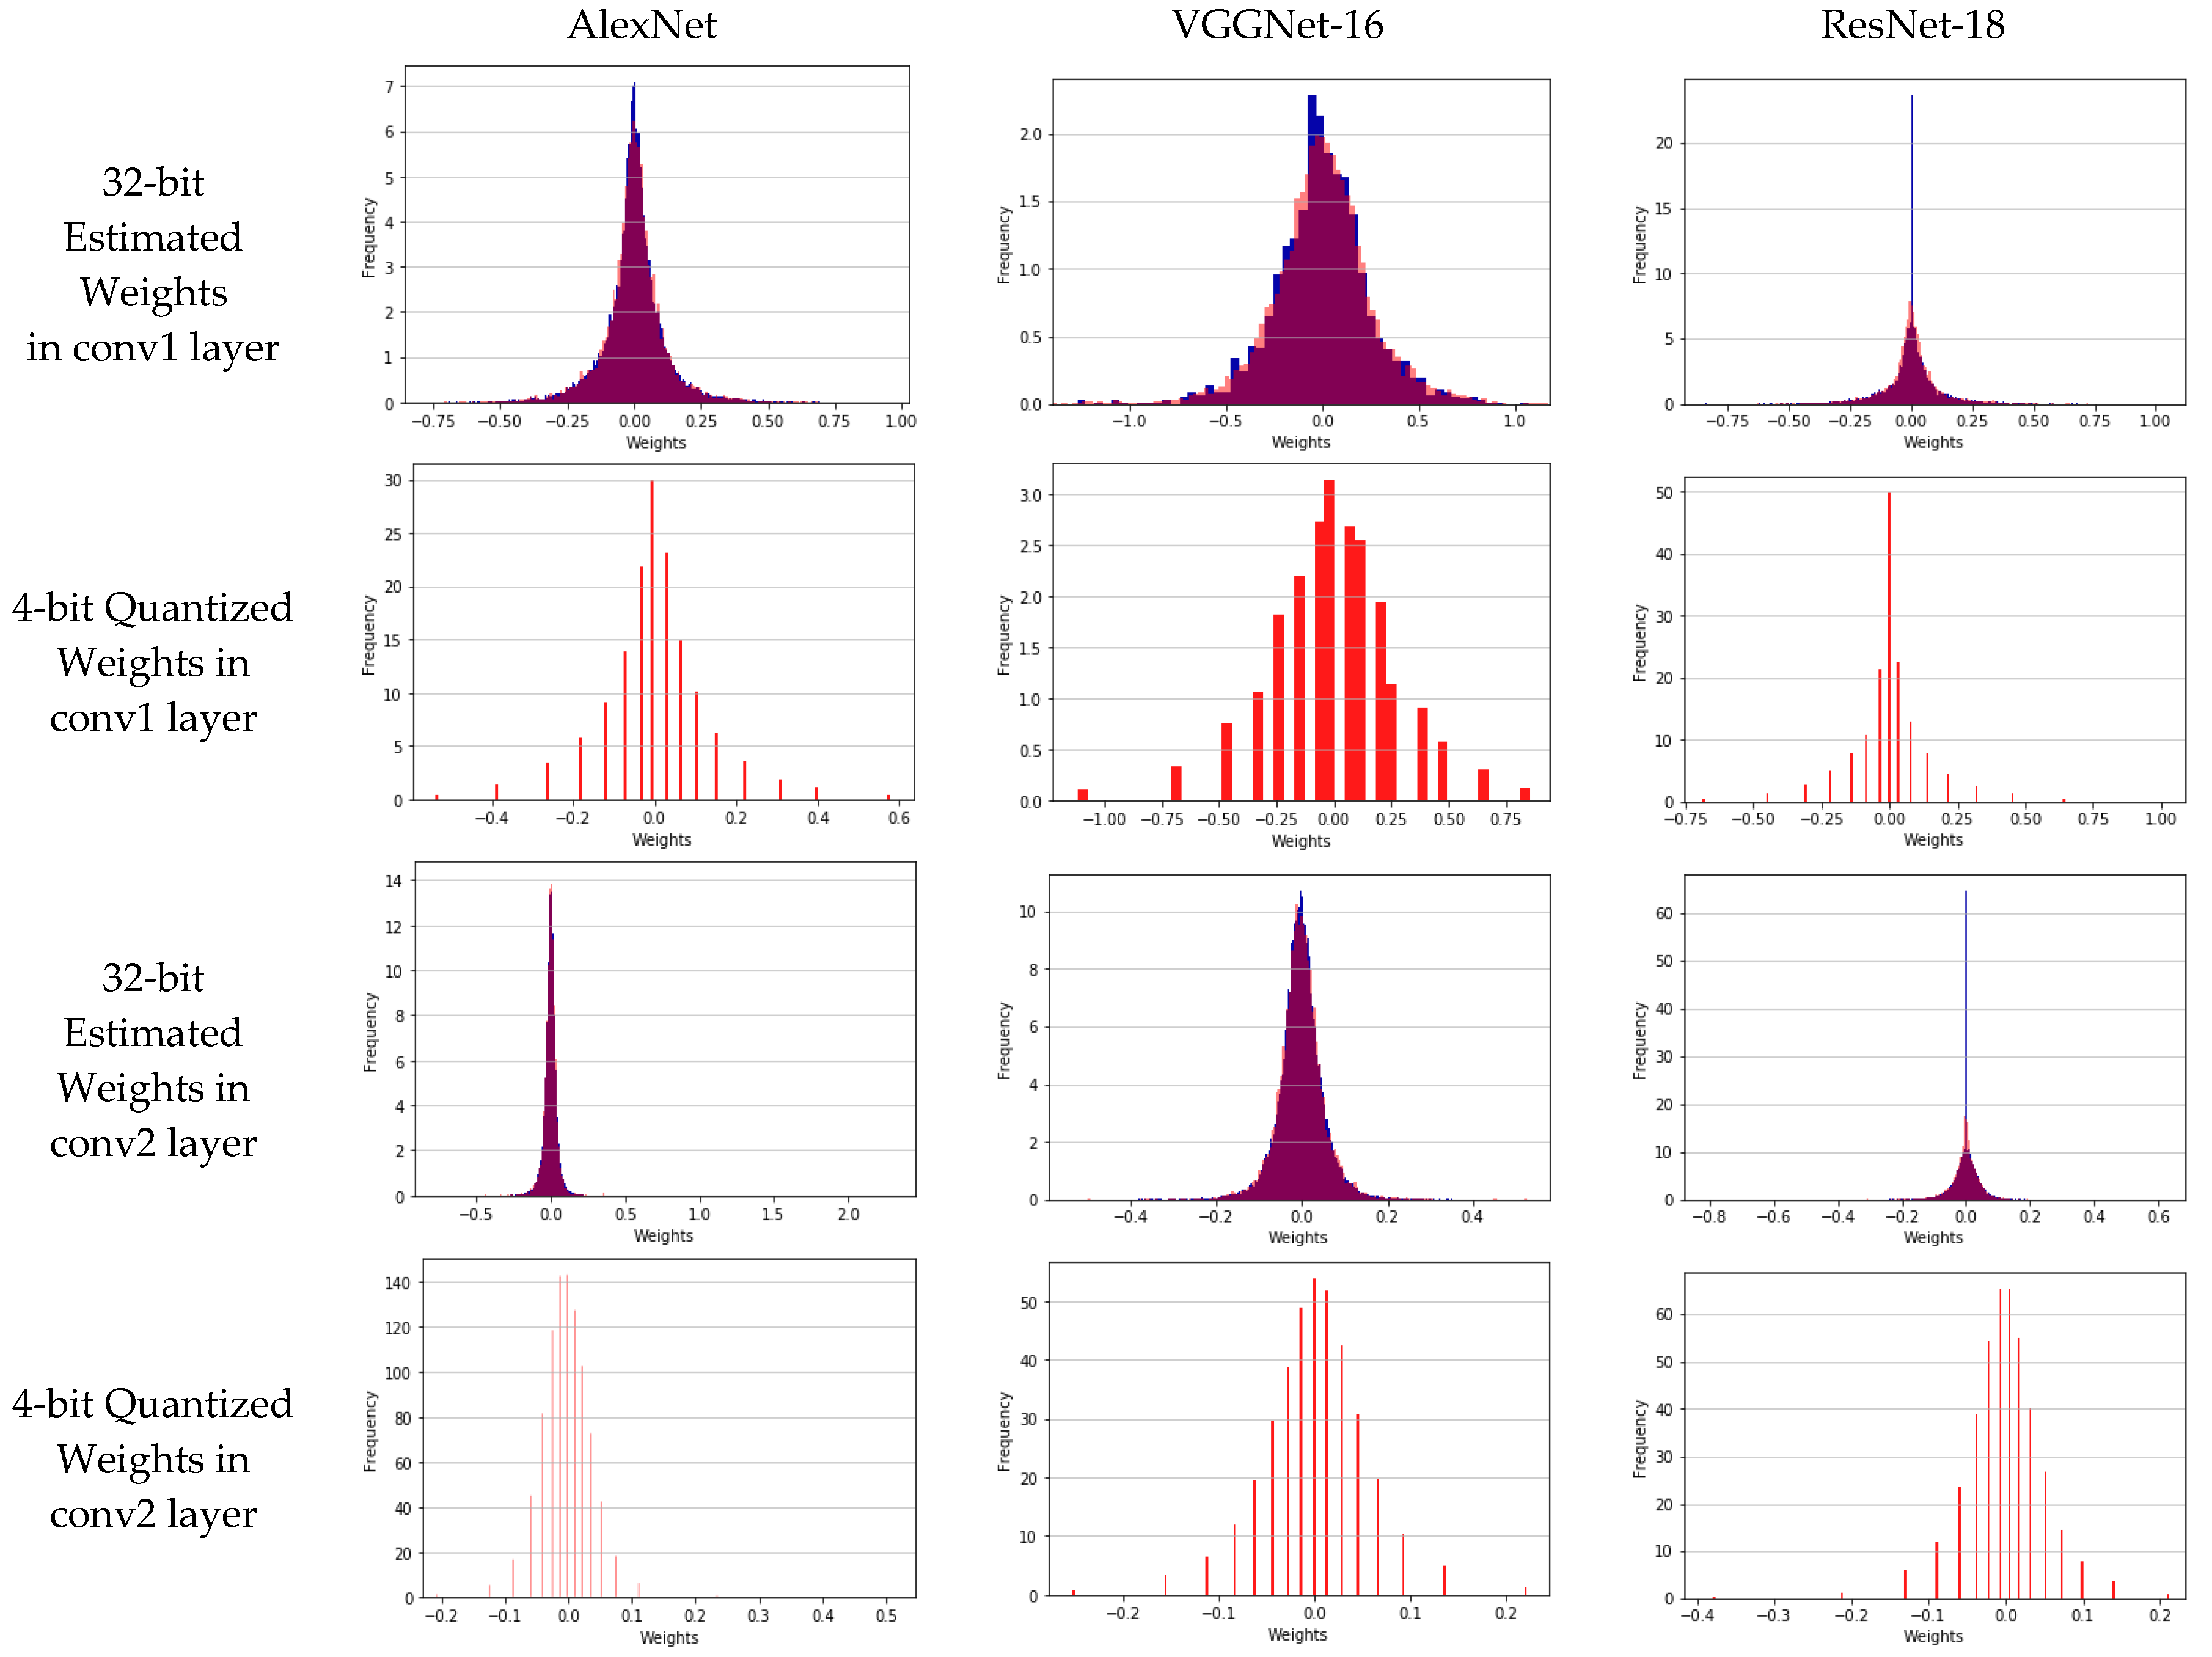
\includegraphics[height=0.8\textheight]{quantization} \\
    \gray{Image Source: \cite{seo_efficient_2019}}
    \large
    Current? SOTA is GPTQ \cite{frantar_gptq_2022}
    \pnote{
        quantization effectively reduces the resolutionof individual weights,
        and can be done while losing very little accuracy
    }
\end{frame}

\subsection{Distillation}
\begin{frame}[c]{Knowledge Distillation}
    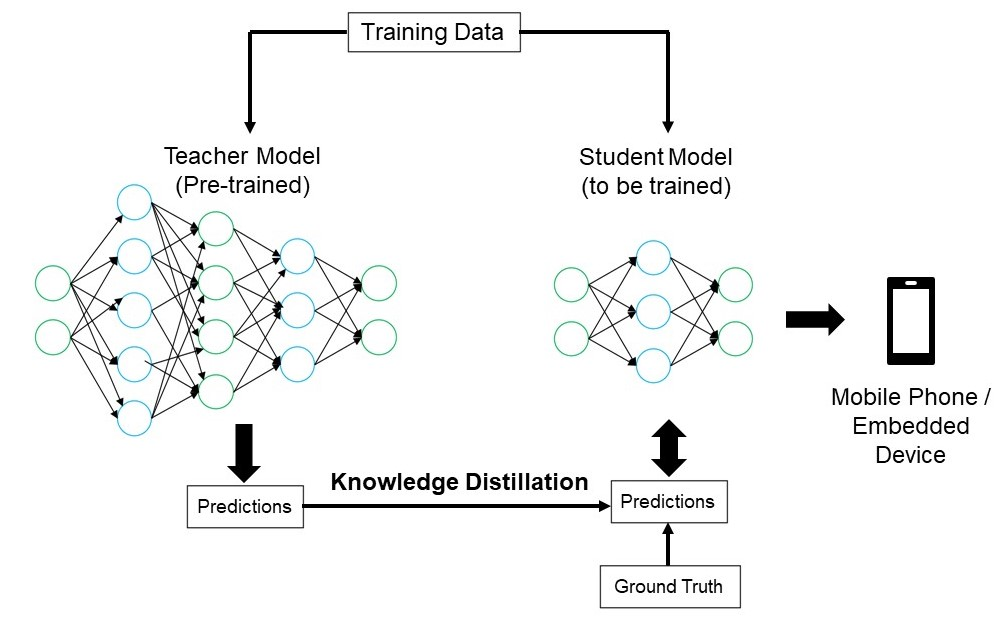
\includegraphics[width=\textwidth]{distillation} \\
    \gray{Image Source: \cite{gou_knowledge_2021}}
    \pnote{
        Distillation can train a student model not just on outputs, \\
        but also intermediate representations, which makes it much \\
        more effective than 'normal' training
    }
\end{frame}

\begin{frame}[c]{Patient Knowledge Distillation}
    \begin{columns}
        \column{0.6\textwidth}
        \begin{minipage}[c][\textheight][c]{\linewidth}
            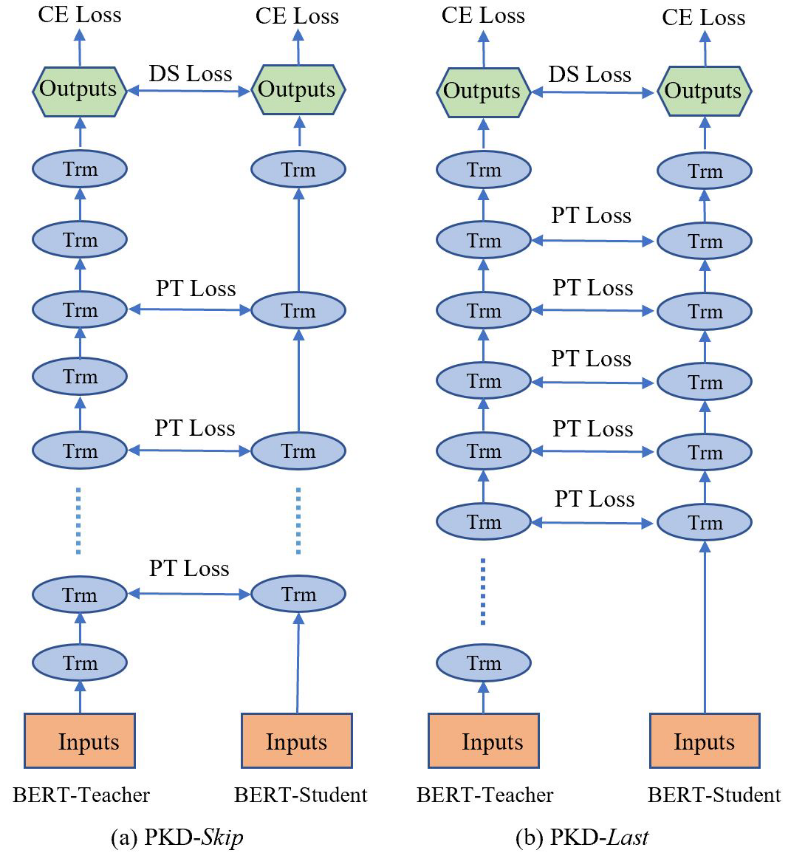
\includegraphics[height=0.8\textheight]{pkd} \\
            \gray{Image Source: \cite{sun_patient_2019}}
        \end{minipage}
        \large
        \column{0.4\textwidth}
        \begin{minipage}[c][\textheight][c]{\linewidth}
            With distillation, size is often \underline{compressed 2-80x} with
            inference speedups of 1.5-10x and keeping $1-\epsilon$ accuracy
            (often 97\%)
        \end{minipage}
    \end{columns}
    \pnote{
        Size compression is particularly relevant for \\
        execution on less powerful hardware \\
        \\
        There are distillation variants where you specify \\
        the accuracy you want to keep.
    }
\end{frame}

\subsection{Rank Reduction}
\begin{frame}[c]{LoRA: Low-Rank Adaptation}
    \begin{columns}
        \column{0.4\textwidth}
        \begin{minipage}[c][\textheight][c]{\linewidth}
            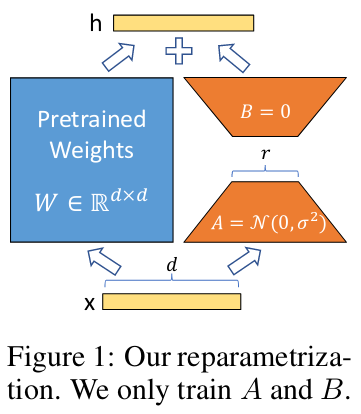
\includegraphics[width=\textwidth]{lora1} \\
            \gray{Image Source: \cite{hu_lora_2021}}
        \end{minipage}
        \column{0.6\textwidth}
        \begin{minipage}[c][.8\textheight][c]{\linewidth}
            \large
            \begin{aquote}{LoRA \cite{hu_lora_2021}}
                LoRA can reduce the number of trainable parameters by 10,000
                times and the GPU memory requirement by 3 times ... despite
                having ... no additional inference latency.
            \end{aquote}
        \end{minipage}
    \end{columns}
    \pnote{
        Has also been successfully used for other architectures
    }
\end{frame}

\begin{frame}[c]{Honorable Mentions}
    \large
    \begin{itemize}[<+(1)->]
        \item Transformer-XL \cite{dai_transformerxl_2019}: Attentive Language Models beyond a Fixed-Length Context
        \item Compressive Transformer \cite{rae_compressive_2019}: Long-Range Sequence Modelling by Compressing Past Memories
        % \item Memorizing Transformer \cite{wu_memorizing_2022}: kNN-augmented attention layer, can reduce parameter count 5x while keeping perplexity
        \item Adaptive Attention Span \cite{sukhbaatar_adaptive_2019}: varying attention distances
        % \item Reflexion \cite{shinn_reflexion_2023}: Asking the model if the answer is correct
        \item Integral Neural Networks \cite{solodskikh_integral}: Use a continuous function to approximate weight landscapes
    \end{itemize}
    \pnote{
        Transformer-XL: requires different positional encoding for previous segments \\
        Compressive: 'summarizing' previous segments \\
        Memorizing: on a layer near the top, using xl-based FIFO compression, can also use external source for that
    }
\end{frame}
